\section{Experimental Results}
\ifCLASSOPTIONonecolumn\begin{figure*}[t]
\centering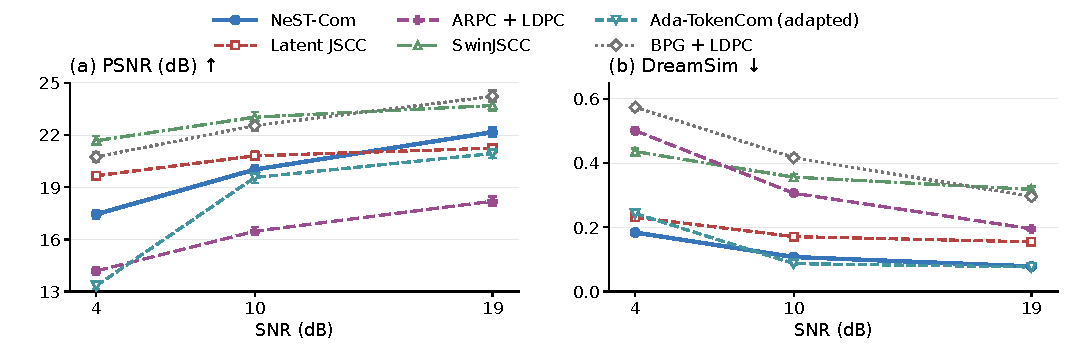
\includegraphics[width=\textwidth]{figure2.pdf}
\caption{Performance on 500 ImageNet validation images at $N=1024$. Error bars show 95\% source-bootstrap confidence intervals. Ada denotes the fixed-frame adaptation.}
\label{fig:performance}
\end{figure*}
\fi
\subsection{Experimental Setup}
We use common500 ImageNet validation images~\cite{imagenet}, a disjoint cal1000 set, and Kodak24~\cite{kodak}, with fixed $256\times256$ preprocessing. ImageNet-calibrated policies remain fixed on Kodak. The six-system main study uses $N=1024$; NeST, WHOLE, and Ada also use $N=512$, each independently calibrated at 4/10/19~dB.

Our convolutional Latent JSCC maps tokenizer latents to symbols and shares $\Dc$, using MSE, LPIPS, and latent-consistency losses. It and SwinJSCC~\cite{swinjscc}, adapted to $256\times256$ and $N{=}1024$, use the same 20\,000 training images and final 100k/200k-update checkpoints. Digital baselines are adaptive BPG~\cite{bpg} + LDPC, ARPC~\cite{arpc} + LDPC with paid captions, and Ada-TokenCom~\cite{adatokencom} adapted to the same fixed single-frame budget. Ada retains LlamaGen-L/VQ16 and prefix arithmetic coding, with a fixed ConvNeXt predicting a paid 10-bit class. Its sampled tail uses CFG=4, $T=1$, top-$k=2000$, and top-$p=1$. Full configurations and training records accompany this letter.

Metrics are PSNR, LPIPS-Alex~\cite{lpips}, DreamSim~\cite{dreamsim}, and CLIP ViT-L/14 image--image cosine (CLIP-I)~\cite{clip}. Frozen FP32 preprocessing uses $224\times224$ bicubic-antialias inputs for DreamSim/CLIP. Three channel outcomes per image, including the gray outputs defined in Sec.~II-C, are averaged before equal-source means and direct source-paired 95\% bootstrap intervals (10\,000 resamples). Endpoint, receiver, and decoding controls use a fixed 100-image subset. Complete four-metric diagnostics and statistical identities are provided in the supplementary material.

\ifCLASSOPTIONonecolumn\else\begin{figure*}[t]
\centering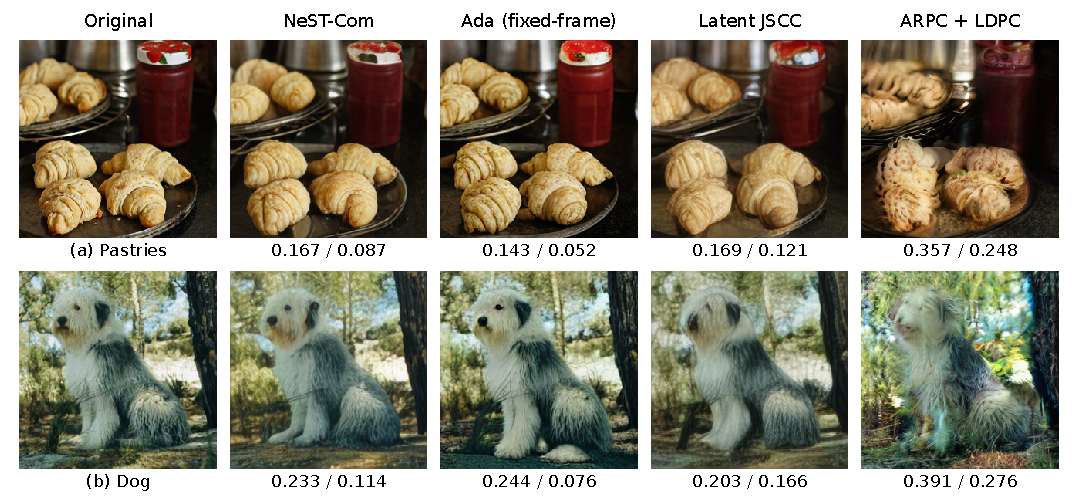
\includegraphics[width=\textwidth]{figure3.pdf}
\caption{Qualitative reconstructions of two development examples at $N=1024$ and 10~dB. Values denote LPIPS-Alex$\downarrow$ / DreamSim$\downarrow$. Ada denotes the fixed-frame adaptation.}
\label{fig:qualitative}
\end{figure*}
\fi
\subsection{Effect of Within-Scale Endpoints}
\begin{table}[t]
\caption{Within-scale endpoint and receiver evidence. (A) Main family-specific policies, PARTIAL minus WHOLE. (B) Fixed 100-source model/MCS/maximum-endpoint control. (C) Ordered interventions on the same 100 sources and actual prefixes. Brackets give source-paired 95\% CIs.}
\label{tab:internal}
\centering\footnotesize
\setlength{\tabcolsep}{2.5pt}
\begin{tabular}{ccc}
\toprule
\multicolumn{3}{l}{(A) Main policies at $N=1024$} \\
SNR & Util. W$\to$P (\%) & $\Delta$PSNR (dB) [95\% CI] \\
\midrule
\multicolumn{3}{l}{common500} \\
4 & 73.81 $\to$ 93.08 & $+0.616\;[0.564,0.673]$ \\
10 & 77.70 $\to$ 95.21 & $+0.701\;[0.637,0.766]$ \\
19 & 85.24 $\to$ 94.73 & $+0.319\;[0.290,0.349]$ \\
\multicolumn{3}{l}{Kodak24} \\
4 & 75.69 $\to$ 93.43 & $+0.396\;[0.236,0.543]$ \\
10 & 78.11 $\to$ 94.99 & $+0.674\;[0.408,0.958]$ \\
19 & 85.69 $\to$ 93.71 & $+0.228\;[0.140,0.324]$ \\
\midrule
\multicolumn{3}{l}{(B) Fixed-granularity diagnostic, 10 dB} \\
Grid (candidates) & Utilization (\%) & PSNR (dB) \\
Whole (7) & 78.15 & 18.952 \\
Half (13) & 89.21 & 19.396 \\
Quarter (25) & 95.38 & 19.612 \\
Eighth (49) & 97.39 & 19.735 \\
\midrule
\multicolumn{3}{l}{(C) Receiver interventions: $\Delta$PSNR (dB) [95\% CI]} \\
SNR & B0$-$A0 & C0$-$B0 \\
10 & $+0.220\;[0.176,0.264]$ & $+0.440\;[0.330,0.558]$ \\
19 & $+0.301\;[0.247,0.358]$ & $+0.000\;[0.000,0.000]$ \\
\bottomrule
\end{tabular}
\par\smallskip\parbox{\columnwidth}{\footnotesize Boundary tokens: A0, unused; B0, residual correction only; C0, residual correction and conditioning update. All three use the received complete coarse scales.}
\end{table}

Table~\ref{tab:internal}(A) compares WHOLE/PARTIAL with shared tokenizer, prior, entropy coder, and $\Dc$. Separate family calibration selects the same MCS at each SNR. Common500 PSNR gains are 0.616/0.701/0.319~dB at 4/10/19~dB. At 10~dB, source-bit utilization rises from 77.70\% to 95.21\% and DreamSim falls by 0.0240. On Kodak, the corresponding PSNR gain is 0.674~dB and DreamSim decreases by 0.0164; its 19~dB DreamSim interval includes zero. The higher utilization retains additional source tokens within the same frame.

Block~B fixes the 100 sources, model, MCS, maximum endpoint, and fitting rule. Whole/Half/Quarter/Eighth grids increase utilization from 78.15\% through 89.21\% and 95.38\% to 97.39\%, with PSNR increasing from 18.952 to 19.735~dB. Relative to the predefined Quarter configuration, Eighth adds $0.123\,[0.079,0.169]$~dB at 10~dB; its DreamSim/CLIP-I difference intervals cross zero.

Block~C applies the boundary-token interventions defined in the table to the same 100 sources and actual received prefixes. The ordered PSNR gains are 0.220 and 0.440~dB at 10~dB, supporting residual correction and the subsequent conditioning update. At 19~dB, the boundary lies in the last scale, so the additional conditioning update has zero effect.

Within the fixed adapted receiver, completion improves the three perceptual measures over coarse-only decoding at both tested low-budget points; complete results are provided in Supplement~S4.

\subsection{Comparison With Existing Methods}
\ifCLASSOPTIONonecolumn\begin{figure*}[t]
\centering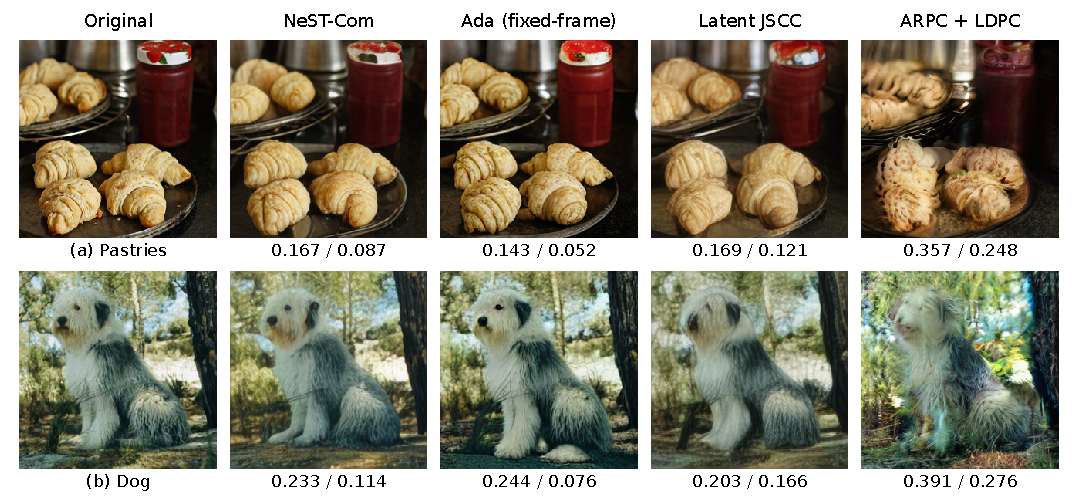
\includegraphics[width=\textwidth]{figure3.pdf}
\caption{Qualitative reconstructions of two development examples at $N=1024$ and 10~dB. Values denote LPIPS-Alex$\downarrow$ / DreamSim$\downarrow$. Ada denotes the fixed-frame adaptation.}
\label{fig:qualitative}
\end{figure*}
\fi
\begin{table}[t]
\caption{Perceptual distance and image-feature similarity on common500 at $N=1024$. Each cell is LPIPS-Alex$\downarrow$ / CLIP-I$\uparrow$. Ada denotes the fixed-frame adaptation. Values are source means.}
\label{tab:external}
\centering\footnotesize
\setlength{\tabcolsep}{3pt}
\begin{tabular}{lccc}
\toprule Method & 4 dB & 10 dB & 19 dB \\
\midrule
NeST-Com & 0.263 / 0.821 & 0.171 / 0.873 & 0.118 / 0.900 \\
Latent JSCC & 0.219 / 0.741 & 0.173 / 0.789 & 0.158 / 0.804 \\
SwinJSCC & 0.530 / 0.627 & 0.469 / 0.669 & 0.440 / 0.697 \\
BPG + LDPC & 0.725 / 0.586 & 0.589 / 0.635 & 0.458 / 0.684 \\
ARPC + LDPC & 0.512 / 0.644 & 0.341 / 0.713 & 0.250 / 0.788 \\
Ada (adapted) & 0.395 / 0.828 & 0.167 / 0.884 & 0.138 / 0.892 \\
\bottomrule
\end{tabular}
\end{table}

Fig.~\ref{fig:performance} and Table~\ref{tab:external} show the complete-system tradeoffs at $N=1024$. NeST exceeds Ada in PSNR by 4.116/0.455/1.226~dB at 4/10/19~dB and exceeds ARPC by 3.26--3.97~dB. Ada has better LPIPS, DreamSim, and CLIP-I at 10~dB, higher CLIP-I at 4~dB, and slightly lower DreamSim at 19~dB. SwinJSCC and BPG have higher PSNR than NeST throughout; Latent JSCC has higher PSNR at 4/10~dB and lower LPIPS at 4~dB. Thus the source-constrained generative route offers a different balance between pixel fidelity and perceptual reconstruction. In the two development examples of Fig.~\ref{fig:qualitative}, Latent JSCC smooths pastry ridges and facial details, while ARPC changes pastry shapes and the dog's pose. NeST and Ada preserve more of these structures but differ in detail; the displayed metric rankings vary by image.

\subsection{Transmission With a Reduced Symbol Budget}
\begin{table}[t]
\caption{Reduced-budget comparison on common500 at $N=512$. Differences are NeST-Com minus the fixed-frame Ada-TokenCom adaptation; brackets give source-paired 95\% CIs. Positive PSNR and negative DreamSim favor NeST-Com.}
\label{tab:reduced}
\centering\footnotesize
\setlength{\tabcolsep}{4pt}
\begin{tabular}{ccc}
\toprule SNR & $\Delta$PSNR (dB) & $\Delta$DreamSim \\
\midrule
4 & $+4.180$ & $-0.1029$ \\
 & $[3.991,4.377]$ & $[-0.1142,-0.0917]$ \\
10 & $+4.055$ & $-0.0660$ \\
 & $[3.880,4.235]$ & $[-0.0747,-0.0573]$ \\
19 & $+1.740$ & $+0.0139$ \\
 & $[1.577,1.909]$ & $[0.0103,0.0173]$ \\
\bottomrule
\end{tabular}
\end{table}

At $N=512$, 68 header symbols leave 444 body symbols. NeST improves over WHOLE by $0.392\,[0.341,0.444]$, $0.399\,[0.356,0.445]$, and $0.792\,[0.740,0.844]$~dB at 4/10/19~dB. All corresponding LPIPS, DreamSim, and CLIP-I paired intervals also favor NeST. At 10~dB, WHOLE and NeST select the same target $(7,0)$ and 16-QAM rate-2/3 MCS. Both fall back from this target for 99.6\% of sources, but NeST retains a within-scale prefix for 89.0\%. The mean number of retained tokens increases from 91.3 to 107.9, raising source-bit utilization from 79.30\% to 93.46\%.

WHOLE already has higher mean PSNR than Ada by 3.79/3.66/0.95~dB. NeST increases these gaps to 4.180/4.055/1.740~dB (Table~\ref{tab:reduced}) and has lower LPIPS at all three SNRs. DreamSim favors NeST at 4/10~dB and Ada at 19~dB; CLIP-I favors Ada throughout.

Replacing Ada's sampled tail by argmax on the fixed 100-image subset leaves NeST higher in PSNR by 4.63/4.60~dB at $N=512$, 4/10~dB; complete sensitivity results are in Supplement~S3.
